\documentclass{article}

%----------------------------------------------------------------
%		Packages
%----------------------------------------------------------------
\usepackage[top=5mm, bottom=2mm, left=0cm, right=0mm, asymmetric, paperwidth=7in, paperheight=7in]{geometry}
\usepackage{tikz}
\usetikzlibrary{shapes.geometric} % Needed for "diamond"

%----------------------------------------------------------------
%		Define Shapes
%----------------------------------------------------------------
\tikzstyle{every node} = [
		font = \scshape\scriptsize, 
		inner xsep = .5cm,
	]

\tikzstyle{event} = [ 
		rectangle,
		rounded corners, 
		minimum height = .5cm, 
		draw = black,
		fill = none,
		text centered
	] 

\tikzstyle{task} = [ 
		rectangle,  
		minimum height = .5cm, 
		draw = black,
		fill = none,
		text centered
	] 
				
\tikzstyle{decision} = [ 
		diamond, 
		aspect = 2,
		draw = black,
		fill = none,
		text centered
	]
	
\tikzstyle{artifact} = [ 
	trapezium, 
	trapezium left angle = 120, 
	trapezium right angle = 60,
	minimum height = .5cm,
	inner xsep = .2cm,
	draw = black,
	fill = none,
	text centered
]

%----------------------------------------------------------------
%		Draw Picture
%----------------------------------------------------------------
\begin{document}

	%------------------------------Picture------------------------------
	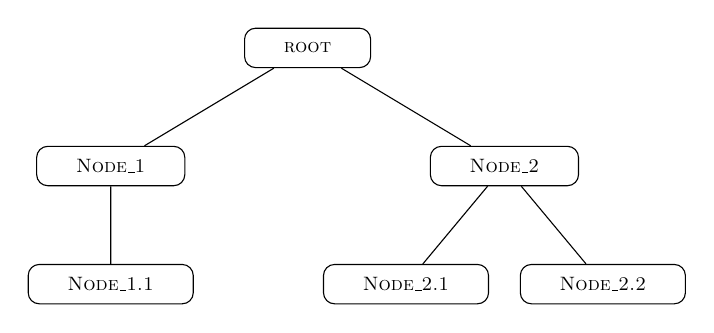
\begin{tikzpicture}[
		level distance = 1.5cm,
		level 1/.style = {sibling distance=5cm}, 
	  level 2/.style = {sibling distance=2.5cm}
	]
	
		%------------------------------Chart------------------------------
		\node [event]{root}
			child {node [event]{Node\_1}
				child {node [event]{Node\_1.1}}}
			child {node [event]{Node\_2}
				child {node [event]{Node\_2.1}}
				child {node [event]{Node\_2.2}}}
		;
 
	\end{tikzpicture}
\end{document}